\begin{frame}[label=title]
	\centering
	\includegraphics[keepaspectratio, width=0.55\textwidth, height=0.48\textheight]{Logos/FreeFlower.pdf}
	\par\medskip
	Informatik: Data Science und Sicherheit\\
	\textbf{Public-Key Kryptologie} \emoji{old-key}\emoji{open-file-folder}
\end{frame}

% \begin{frame}[fragile]{Schwäche von VIGENÈRE}
% Angenommen wir haben einen Klartext, der aus genau 1000 Buchstaben besteht.
% \begin{itemize}
%   \item VIGENÈRE-Schlüssel der Länge 5: Bilde 5 \textit{Gruppen}, bestehend aus jeweils 200 Buchstaben. Führe innerhalb jeder Gruppe eine Häufigkeitsanalyse (wie bei CAESAR) durch. (sehr einfach angreifbar)
%   \item VIGENÈRE-Schlüssel der Länge 50: Bilde 50 \textit{Gruppen}, bestehend aus jeweils 20 Buchstaben. Eine Häufigkeitsanalye innerhalb der Gruppen wird hier höchst unzuverlässig. (Kryptoanalyse wenig realistisch)
% \end{itemize}
% \end{frame}
%
% \begin{frame}[fragile]{vom VIGENÈRE zum One-Time-Pad}
%   Idee \emoji{light-bulb}:
%   \begin{itemize}
%     \item Verwende einen Schlüssel, der (mindestens) so lange ist wie der Klartext!
%     \item Wähle jeden Buchstaben des Schlüssels vollkommen zufällig!
%     \item Verwende diesen Schlüssel nur einmal (Begründung: siehe weiter unten).
%   \end{itemize}
% \end{frame}
%
%
% \begin{frame}{One-Time-Pad}
%  \begin{myBox}[ONE-TIME-PAD, Frank Miller (1882)]{mybox:onetime}
% \begin{enumerate}
%   \item Erzeuge einen Schlüssel der (mindestens) so lange ist wie der Klartext. Jeder einzelne Buchstabe des Schlüssels muss vollkommen zufällig gewählt werden.
%   \item Der Schlüssel darf nicht mehrfach verwendet werden (nicht einmal Teile des Schlüssels).
%   \item Der Schlüssel muss von den kommunizierenden Parteien geheim gehalten werden.
% \end{enumerate}
% \end{myBox}
% \end{frame}
%
%
% \begin{frame}{Sicht des Angreifers}
%   Ein Angreifer fängt den Kryptotext ab. Was lernt dieser Angreifer aus dem Kryptotext?
%   \begin{itemize}
%     \item Jeder Buchstabe des Kryptotexts entsteht durch eine zufällige Verschiebung des entsprechenden Buchstabens im Klartext.
%     \item Damit ist der Kryptotext nichts anderes als eine zufällige Folge von Buchstaben.
%     \item Der Angreifer lernt lediglich eine obere Schranke für die Länge des Klartextes. (ist der Kryptotext $n$ Zeichen lang, kann der Klartext offensichtlich höchstens aus $n$ Zeichen bestehen)
%   \end{itemize}
% \end{frame}

\begin{frame}[t]{Alice erzeugt ihr Schlüsselpaar}
	\begin{itemize}
		\item Alice generiert ein Paar von Schlüsseln: einen öffentlichen Schlüssel und einen privaten Schlüssel (Geheimnis), welche miteinander in einem Zusammenhang stehen.
		\item Den öffentlichen Schlüssel macht sie öffentlich bekannt. Den privaten Schlüssel muss sie für sich behalten.
	\end{itemize}
\end{frame}

\begin{frame}[t]{Bob sendet eine Nachricht an Alice}
	\small
	\begin{itemize}
		\item Bob möchte eine verschlüsselte Nachricht an Alice senden.
		\item Dazu nimmt er sich (eine Kopie) ihres öffentlichen Schlüssels und verwendet diesen um die Nachricht zu verschlüsseln.
		\item Die (mit Hilfe von ihrem öffentlichen Schlüssel) verschlüsselte Nachricht sendet er dann Alice.
		\item Diese verschlüsselte Nachricht kann Alice mit Hilfe ihres privaten Schlüssels (Geheimnisses) sehr einfach entschlüsseln.
		\item Ein Angreifer (Abhörer) müsste für die Entschlüsslung einen astronomischen Aufwand betreiben.
	\end{itemize}
\end{frame}

\begin{frame}{Alices öffentlicher Schlüssel}
	\begin{columns}[c,onlytextwidth]
		\begin{column}{0.48\textwidth}
			In unserem Beispiel ist der öffentliche Schlüssel von Alice der folgende Graph:
		\end{column}
		\begin{column}{0.48\textwidth}
			\centering
			\adjustbox{width=\linewidth,max totalheight=0.65\textheight}{%
				\begin{tikzpicture}[shorten >=1pt,auto,node distance=3cm, semithick, scale=0.1]
					\tikzstyle{every state}=[text=black]
					\node[state] (A) {}             ;
					\node[state] (B) [right of=A] {};
					\node[state] (C) [below right of=A] {};
					\node[state] (D) [below left of=A] {};
					\node[state] (E) [right of=C] {};
					\node[state] (F) [below of=D] {};
					\node[state] (G) [below right of=C] {};

					\path (A) edge (B)
					(A) edge (D)
					(A) edge (C)
					(B) edge (C)
					(B) edge (E)
					(C) edge (E)
					(D) edge (F)
					(F) edge (G)
					(E) edge (G)
					;
				\end{tikzpicture}
			} %
			% \label{fig:Knobel}
		\end{column}
	\end{columns}
\end{frame}

\begin{frame}{Verschlüsselung: Geheime Zahlen wählen}
	\begin{columns}[c,onlytextwidth]
		\begin{column}{0.48\textwidth}
			\small
			Bob möchte die Nachricht (Klartext, geheime Zahl) \green{31} an Alice übermitteln. Dazu verwendet er ihren öffentlichen Schlüssel (Graphen). Er wählt die schwarzen Zahlen in den Knoten so, dass deren Summe genau der Nachricht \green{31} entspricht. Diese schwarzen Zahlen muss Bob geheim behalten.

			\[
				5 + 17 + 3 - 11 + 14 - 2 + 5 = \green{31}
			\]
		\end{column}
		\begin{column}{0.48\textwidth}
			\centering
			\adjustbox{width=\linewidth,max totalheight=0.65\textheight}{%
				\begin{tikzpicture}[shorten >=1pt,auto,node distance=3cm, semithick, scale=0.1]
					\tikzstyle{every state}=[text=black]
					\node[state] (A) {5}             ;
					\node[state] (B) [right of=A] {17};
						\node[state] (C) [below right of=A] {-11};
						\node[state] (D) [below left of=A] {3};
					\node[state] (E) [right of=C] {14};
					\node[state] (F) [below of=D] {-2};
					\node[state] (G) [below right of=C] {5};

					\path (A) edge (B)
					(A) edge (D)
					(A) edge (C)
					(B) edge (C)
					(B) edge (E)
					(C) edge (E)
					(D) edge (F)
					(F) edge (G)
					(E) edge (G)
					;
				\end{tikzpicture}
			} %
			% \caption*{(a)}
			% \label{fig:Knobel}
		\end{column}
	\end{columns}
\end{frame}

\begin{frame}{Verschlüsselung: Nachbarsummen berechnen}
	\begin{columns}[c,onlytextwidth]
		\begin{column}{0.48\textwidth}
			\small
			Bob berechnet die \red{roten} Zahlen. Die rote Zahl in dem Knoten $i$ ist die Summe der schwarzen Zahlen des Knoten $i$ selbst und aller seiner Nachbarn. Bob muss nun diese schwarzen Zahlen aus dem Graphen löschen.
		\end{column}
		\begin{column}{0.48\textwidth}
			\centering
			\adjustbox{width=\linewidth,max totalheight=0.65\textheight}{%
				\begin{tikzpicture}[shorten >=1pt,auto,node distance=3cm, semithick, scale=0.1]
					\tikzstyle{every state}=[text=black]
					\node[state,align=center] (A) {$5$\\$\red{(14)}$}             ;
					\node[state,align=center] (B) [right of=A] {$17$\\$\red{(25)}$};
					\node[state,align=center] (C) [below right of=A] {$-11$\\$\red{(25)}$};
					\node[state,align=center] (D) [below left of=A] {$3$\\$\red{(6)}$};
					\node[state,align=center] (E) [right of=C] {$14$\\$\red{(25)}$};
					\node[state,align=center] (F) [below of=D] {$-2$\\$\red{(6)}$};
					\node[state,align=center] (G) [below right of=C] {$5$\\$\red{(17)}$};

					\path (A) edge (B)
					(A) edge (D)
					(A) edge (C)
					(B) edge (C)
					(B) edge (E)
					(C) edge (E)
					(D) edge (F)
					(F) edge (G)
					(E) edge (G)
					;
				\end{tikzpicture}
			} %
			% \caption*{(a)}
			% \label{fig:Knobel}
		\end{column}
	\end{columns}
\end{frame}

\begin{frame}{Verschlüsselung: Nachricht an Alice senden}
	\begin{columns}[c,onlytextwidth]
		\begin{column}{0.48\textwidth}
			Der folgende Graph mit den roten Zahlen ist nun die verschlüsselte Nachricht, welche Bob an Alice (über einen unsicheren Kanal) senden darf:
		\end{column}
		\begin{column}{0.48\textwidth}
			\centering
			\adjustbox{width=\linewidth,max totalheight=0.65\textheight}{%
				\begin{tikzpicture}[shorten >=1pt,auto,node distance=3cm, semithick, scale=0.1]
					\tikzstyle{every state}=[text=black]
					\node[state,align=center] (A) {$\red{14}$}             ;
					\node[state,align=center] (B) [right of=A] {$\red{25}$};
					\node[state,align=center] (C) [below right of=A] {$\red{25}$};
					\node[state,align=center] (D) [below left of=A] {$\red{6}$};
					\node[state,align=center] (E) [right of=C] {$\red{25}$};
					\node[state,align=center] (F) [below of=D] {$\red{6}$};
					\node[state,align=center] (G) [below right of=C] {$\red{17}$};

					\path (A) edge (B)
					(A) edge (D)
					(A) edge (C)
					(B) edge (C)
					(B) edge (E)
					(C) edge (E)
					(D) edge (F)
					(F) edge (G)
					(E) edge (G)
					;
				\end{tikzpicture}
			} %
			% \caption*{(a)}
			% \label{fig:Knobel}
		\end{column}
	\end{columns}
\end{frame}

\begin{frame}[t,label=repetition]{Dominating Set}
	\begin{mydefinition}[Dominating Set]\label{mydefinition:DominatingSet}
		Sei $G = (V, E)$ ein Graph.
		\begin{itemize}
			\item Ein Knoten $i$ \tib{dominiert} einen Knoten $j$ falls $i = j$ (ein Knoten dominiert sich selbst) oder falls eine Kante von $i$ nach $j$ existiert.
			\item Eine Teilmenge $S\subseteq V$ heisst \tib{Dominating Set} (DS) von $G$, falls jeder Knoten von $G$ von mindestens einem Knoten in $S$ dominiert wird.
		\end{itemize}
	\end{mydefinition}
\end{frame}

\begin{frame}[t]{Perfect Dominating Set}
	\begin{mydefinition}[Perfect Dominating Set]
		Ein Dominating Set wird \tib{perfect} (PDS) genannt, falls jeder Knoten von $G$ von genau einem Knoten in $S$ dominiert wird.
	\end{mydefinition}
\end{frame}

\begin{frame}{Dominating Sets im Vergleich}
	\begin{figure}
		\centering
		\begin{subfigure}[b]{0.3\textwidth}
			\adjustbox{width=0.95\linewidth,max totalheight=0.34\textheight}{%
				\begin{tikzpicture}[shorten >=1pt,auto,node distance=3cm, semithick, scale=0.1]
					\tikzstyle{every state}=[text=black]
					\node[state] (A) {}             ;
					\node[state,fill=Red,draw=Red] (B) [below right of=A] {};
					\node[state,fill=Red,draw=Red] (C) [above right of=A] {};
					\node[state,fill=Red,draw=Red] (D) [right of=C] {};
					\node[state] (E) [right of=B] {};
					\node[state] (F) [right of=D] {};

					\path (A) edge (C)
					(A) edge (B)
					(B) edge (C)
					(B) edge (E)
					(C) edge (D)
					(D) edge (E)
					(D) edge (F)
					;
				\end{tikzpicture}
			} %
			\caption*{(a)}
			\label{fig:aDominatingSets}
		\end{subfigure}
		\hfill
		\begin{subfigure}[b]{0.3\textwidth}
			\adjustbox{width=0.95\linewidth,max totalheight=0.34\textheight}{%
				\begin{tikzpicture}[shorten >=1pt,auto,node distance=3cm, semithick, scale=0.1]
					\tikzstyle{every state}=[text=black]
					\node[state] (A) {}             ;
					\node[state] (B) [below right of=A] {};
					\node[state,fill=Red,draw=Red] (C) [above right of=A] {};
					\node[state,fill=Red,draw=Red] (D) [right of=C] {};
					\node[state] (E) [right of=B] {};
					\node[state] (F) [right of=D] {};

					\path (A) edge (C)
					(A) edge (B)
					(B) edge (C)
					(B) edge (E)
					(C) edge (D)
					(D) edge (E)
					(D) edge (F)
					;
				\end{tikzpicture}
			} %
			\caption*{(b)}
			\label{fig:bDominatingSets}
		\end{subfigure}
		\hfill
		\begin{subfigure}[b]{0.3\textwidth}
			\adjustbox{width=0.95\linewidth,max totalheight=0.34\textheight}{%
				\begin{tikzpicture}[shorten >=1pt,auto,node distance=3cm, semithick, scale=0.1]
					\tikzstyle{every state}=[text=black]
					\node[state] (A) {}             ;
					\node[state,fill=Red,draw=Red] (B) [below right of=A] {};
					\node[state] (C) [above right of=A] {};
					\node[state] (D) [right of=C] {};
					\node[state] (E) [right of=B] {};
					\node[state,fill=Red,draw=Red] (F) [right of=D] {};

					\path (A) edge (C)
					(A) edge (B)
					(B) edge (C)
					(B) edge (E)
					(C) edge (D)
					(D) edge (E)
					(D) edge (F)
					;
				\end{tikzpicture}
			} %
			\caption*{(c)}
			\label{fig:cDominatingSets}
		\end{subfigure}
		\caption{Die roten Knoten in (a) und (b) stellen Dominating Sets (aber keine perfect Dominating Sets) im jeweiligen Graphen dar. Die roten Knoten in (c) formen sogar ein perfect Dominating Set.}
	\end{figure}
\end{frame}

\begin{frame}{Schlüsselgenerierung (1/4): Knoten anlegen}
	\begin{columns}[c,onlytextwidth]
		\begin{column}{0.48\textwidth}
			Beginne mit einigen Knoten.
		\end{column}
		\begin{column}{0.48\textwidth}
			\centering
			\adjustbox{width=\linewidth,max totalheight=0.65\textheight}{%
				\begin{tikzpicture}[shorten >=1pt,auto,node distance=3cm, semithick, scale=0.1]
					\tikzstyle{every state}=[text=black]
					\node[state] (A) {}             ;
					\node[state] (B) [right of=A] {};
					\node[state] (C) [below right of=A] {};
					\node[state] (D) [below left of=A] {};
					\node[state] (E) [right of=C] {};
					\node[state] (F) [below of=D] {};
					\node[state] (G) [below right of=C] {};

					%   \path (A) edge (B)
					%   (A) edge (D)
					%   (A) edge (C)
					%   (B) edge (C)
					%   (B) edge (E)
					%   (D) edge (F)
					%   (F) edge (G)
					%   (E) edge (G)
					% ;
				\end{tikzpicture}
			} %
			% \caption*{(a)}
			% \label{fig:Knobel}
		\end{column}
	\end{columns}
\end{frame}


\begin{frame}{Schlüsselgenerierung (2/4): PDS wählen}
	\begin{columns}[c,onlytextwidth]
		\begin{column}{0.48\textwidth}
			Wähle die Knoten, welche zum PDS gehören sollen.
		\end{column}
		\begin{column}{0.48\textwidth}
			\centering
			\adjustbox{width=\linewidth,max totalheight=0.65\textheight}{%
				\begin{tikzpicture}[shorten >=1pt,auto,node distance=3cm, semithick, scale=0.1]
					\tikzstyle{every state}=[text=black]
					\node[state] (A) {}             ;
					\node[state] (B) [right of=A] {};
					\node[state] (C) [below right of=A] {};
					\node[state,fill=Red,draw=Red] (D) [below left of=A] {};
					\node[state,fill=Red,draw=Red] (E) [right of=C] {};
					\node[state] (F) [below of=D] {};
					\node[state] (G) [below right of=C] {};

					%   \path (A) edge (B)
					%   (A) edge (D)
					%   (A) edge (C)
					%   (B) edge (C)
					%   (B) edge (E)
					%   (D) edge (F)
					%   (F) edge (G)
					%   (E) edge (G)
					% ;
				\end{tikzpicture}
			} %
			% \caption*{(a)}
			% \label{fig:Knobel}
		\end{column}
	\end{columns}
\end{frame}

\begin{frame}{Schlüsselgenerierung (3/4): Knoten verbinden}
	\begin{columns}[c,onlytextwidth]
		\begin{column}{0.48\textwidth}
			Verbinde jeden Knoten, der nicht im PDS liegt mit genau einem Knoten aus dem PDS.
		\end{column}
		\begin{column}{0.48\textwidth}
			\centering
			\adjustbox{width=\linewidth,max totalheight=0.65\textheight}{%
				\begin{tikzpicture}[shorten >=1pt,auto,node distance=3cm, semithick, scale=0.1]
					\tikzstyle{every state}=[text=black]
					\node[state] (A) {}             ;
					\node[state] (B) [right of=A] {};
					\node[state] (C) [below right of=A] {};
					\node[state,fill=Red,draw=Red] (D) [below left of=A] {};
					\node[state,fill=Red,draw=Red] (E) [right of=C] {};
					\node[state] (F) [below of=D] {};
					\node[state] (G) [below right of=C] {};

					\path %(A) edge (B)
					(A) edge (D)
					%   (A) edge (C)
					%   (B) edge (C)
					(B) edge (E)
					(C) edge (E)
					(D) edge (F)
					%   (F) edge (G)
					(E) edge (G)
					;
				\end{tikzpicture}
			} %
			% \caption*{(a)}
			% \label{fig:Knobel}
		\end{column}
	\end{columns}
\end{frame}

\begin{frame}{Schlüsselgenerierung (4/4): Kanten ergänzen}
	\begin{columns}[c,onlytextwidth]
		\begin{column}{0.48\textwidth}
			\small
			Füge zur Verschleierung weitere Kanten zwischen den Knoten, welche nicht zum PDS gehören, hinzu. Zeichne also keine weiteren Kanten, welche in den roten Knoten beginnen / enden! Der Graph ist ihr öffentlicher Schlüssel. Die beiden roten Knoten (perfect dominating set) ist ihr privater Schlüssel.
		\end{column}
		\begin{column}{0.48\textwidth}
			\centering
			\adjustbox{width=\linewidth,max totalheight=0.65\textheight}{%
				\begin{tikzpicture}[shorten >=1pt,auto,node distance=3cm, semithick, scale=0.1]
					\tikzstyle{every state}=[text=black]
					\node[state] (A) {}             ;
					\node[state] (B) [right of=A] {};
					\node[state] (C) [below right of=A] {};
					\node[state,fill=Red,draw=Red] (D) [below left of=A] {};
					\node[state,fill=Red,draw=Red] (E) [right of=C] {};
					\node[state] (F) [below of=D] {};
					\node[state] (G) [below right of=C] {};

					\path (A) edge (B)
					(A) edge (D)
					(A) edge (C)
					(B) edge (C)
					(B) edge (E)
					(C) edge (E)
					(D) edge (F)
					(F) edge (G)
					(E) edge (G)
					;
				\end{tikzpicture}
			} %
			% \caption*{(a)}
			% \label{fig:Knobel}
		\end{column}
	\end{columns}
\end{frame}

\begin{frame}{Angriff mit einem linearen Gleichungssystem}
	\begin{columns}[c,onlytextwidth]
		\begin{column}{0.48\textwidth}
			\centering
			\adjustbox{width=\linewidth,max totalheight=0.65\textheight}{%
				\begin{tikzpicture}[shorten >=1pt,auto,node distance=3cm, semithick, scale=0.1]
					\tikzstyle{every state}=[text=black]

					\node[state,align=center] (A) {\textcolor{red}{14}\\\(\mathit{A}\)};
					\node[state,align=center] (B) [right of=A] {\textcolor{red}{25}\\\(\mathit{B}\)};
					\node[state,align=center] (C) [below right of=A] {\textcolor{red}{25}\\\(\mathit{C}\)};
					\node[state,align=center] (D) [below left of=A] {\textcolor{red}{6}\\\(\mathit{D}\)};
					\node[state,align=center] (E) [right of=C] {\textcolor{red}{25}\\\(\mathit{E}\)};
					\node[state,align=center] (F) [below of=D] {\textcolor{red}{6}\\\(\mathit{F}\)};
					\node[state,align=center] (G) [below right of=C] {\textcolor{red}{17}\\\(\mathit{G}\)};

					\path (A) edge (B)
					(A) edge (D)
					(A) edge (C)
					(B) edge (C)
					(B) edge (E)
					(C) edge (E)
					(D) edge (F)
					(F) edge (G)
					(E) edge (G)
					;
				\end{tikzpicture}
			} %
		\end{column}
		\begin{column}{0.48\textwidth}
			\small
			\[
				\begin{aligned}
					(1) \quad        & 14 = A + B + C + D \\
					(2) \quad        & 25 = A + B + C + E \\
					\blue{(3)} \quad & 25 = A + B + C + E \\
					(4) \quad        & 6  = A + D + F     \\
					(5) \quad        & 25 = B + C + E + G \\
					(6) \quad        & 6  = D + F + G     \\
					(7) \quad        & 17 = E + F + G     \\
				\end{aligned}
			\]
		\end{column}
	\end{columns}
\end{frame}

\begin{frame}{Was bedeutet eine Lösung des Gleichungssystems?}
	Eine \textbf{Lösung} legt für \textbf{alle sieben Unbekannten}
	$A, B, C, D, E, F, G$ je eine Zahl fest. Setzt man diese Zahlen ein,
	müssen \textbf{alle sieben Gleichungen gleichzeitig stimmen}.

	\medskip
	In unserem Beispiel sind unter anderem diese beiden Belegungen möglich:
	\begin{center}
		\begin{tabular}{lrrrrrrr}
			\toprule
			& $A$ & $B$ & $C$ & $D$ & $E$ & $F$ & $G$ \\
			\midrule
			Bobs Zahlen & 5 & 17 & $-11$ & 3 & 14 & $-2$ & 5 \\
			Andere Lösung & 5 & 6 & 0 & 3 & 14 & $-2$ & 5 \\
			\bottomrule
		\end{tabular}
	\end{center}
	Beide Belegungen ergeben dieselben roten Nachbarsummen.
	Bei $B$ und $C$ ist jeweils nur die gemeinsame Summe $B+C=6$ entscheidend.
\end{frame}

\begin{frame}{Redundante Gleichungen: Die Summe bleibt eindeutig}
	\begin{itemize}
		\item Die Gleichungen (2) und (3) sind identisch: Die Wiederholung liefert keine zusätzliche Information.
		\item Die Nachricht ist die \textbf{Summe aller sieben Knotenzahlen}. Addiert man (4) und (5), erhält man:
	\end{itemize}
	\[
		\begin{aligned}
			6 &= A + D + F, \\
			25 &= B + C + E + G, \\[2pt]
			\green{31} &= A + B + C + D + E + F + G.
		\end{aligned}
	\]
	Jede Zahlenbelegung, die alle Gleichungen erfüllt, hat somit die Gesamtsumme \green{31}. Das gilt auch für die beiden Belegungen auf der vorherigen Folie.
\end{frame}

\begin{frame}{Warum ist die Summe immer eindeutig?}
	\small
	Die folgende Überlegung gilt für jeden Graphen dieses Verfahrens, der ein PDS besitzt:
	\begin{enumerate}
		\item Betrachte irgendeine Zahlenbelegung, die alle Gleichungen erfüllt. Jede rote Zahl ist dann die Summe der eingesetzten Zahl am eigenen Knoten und der Zahlen seiner Nachbarn.
		\item Addiert Alice die roten Zahlen an den PDS-Knoten, zählt sie deshalb die eingesetzten Zahlen in deren Nachbarschaften mit, jeweils einschliesslich des PDS-Knotens selbst.
		\item Beim PDS gehört jeder Knoten zu \textbf{genau einer} solchen Nachbarschaft. Jede eingesetzte Zahl wird also \textbf{genau einmal} gezählt.
	\end{enumerate}
	\[
		\begin{gathered}
			\text{Summe aller eingesetzten}\\
			\text{Knotenzahlen}
		\end{gathered}
		=
		\begin{gathered}
			\text{Summe der roten Zahlen}\\
			\text{an den PDS-Knoten}
		\end{gathered}
	\]
	Die rechte Seite ist durch die übermittelten roten Zahlen festgelegt.
	Deshalb ist die linke Seite bei jeder passenden Zahlenbelegung gleich.
\end{frame}

\begin{frame}{Wie nutzt ein Angreifer diese Eigenschaft?}
	\begin{enumerate}
		\item Aus dem öffentlichen Graphen und den roten Zahlen stellt er das Gleichungssystem auf.
		\item Mit dem Gauss-Verfahren findet er \textbf{eine} Zahlenbelegung, die alle Gleichungen erfüllt. Falls Variablen frei wählbar bleiben, kann er dafür beispielsweise $0$ einsetzen und die übrigen Zahlen daraus berechnen.
		\item Er addiert alle gefundenen Knotenzahlen. Diese Summe ist die \textbf{geheime Nachricht}.
	\end{enumerate}
	\medskip
	Er muss weder Bobs ursprüngliche Zahlen noch das geheime PDS kennen.
	Die PDS-Eigenschaft garantiert, dass jede passende Belegung dieselbe Summe liefert.
\end{frame}

\begin{frame}{Rechenaufwand des Gauss-Verfahrens}
	\centering
	% Auch Achsenbeschriftungen in die Grössenbegrenzung einbeziehen.
	\adjustbox{max width=\linewidth,max totalheight=0.72\textheight}{%
		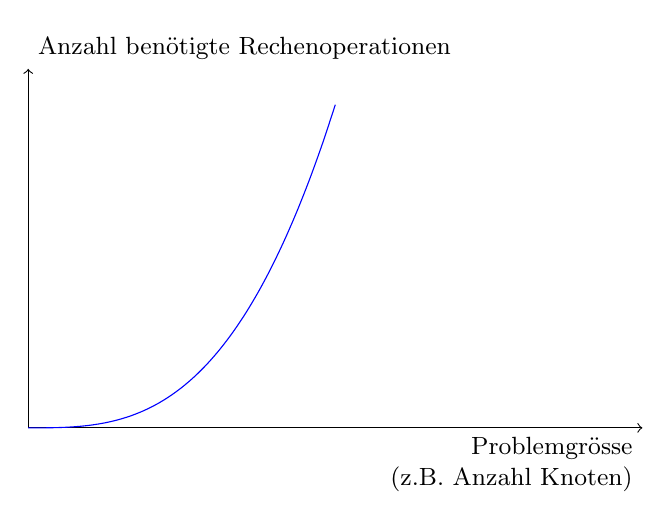
\begin{tikzpicture}[x=0.65cm,y=0.38cm]
			% \draw[style=help lines] (-7.9,-7.9) grid (7.9,7.9);
			%[step=0.5cm]      (-6.9,-6.9) grid (6.9,6.9);

			\draw[->] (0,0) -- (12,0) node[below left,align=right,font=\small] {Problemgrösse\\(z.B. Anzahl Knoten)};
			\draw[->] (0,0) -- (0,12) node[above right,font=\small] {Anzahl benötigte Rechenoperationen};
			\draw[domain=0:6, smooth, variable=\x, blue] plot ({\x}, {0.05*\x*\x*\x});


			% {\tiny
			% \foreach \x/\xtext in {-7,-6,-5,-4,-3,-2,-1,1,2,3,4,5,6,7}
			% \draw[shift={(\x,0)}] (0pt,2pt) -- (0pt,-2pt) node[below] {$\xtext$};
			%
			% \foreach \y/\ytext in {-7,-6,-5,-4,-3,-2,-1,1,2,3,4,5,6,7}
			% \draw[shift={(0,\y)}] (2pt,0pt) -- (-2pt,0pt) node[left] {$\ytext$};
			% }
			%
			% \draw [fill] (0,0) circle [radius=.1];
			% \draw [fill] (4,2) circle [radius=.1];
		\end{tikzpicture}
	}
\end{frame}

% \begin{frame}{Binäres One-Time-Pad (Bin-OTP)}
	Beim \textbf{Bin-OTP} arbeiten wir nicht mit dem lateinischen Alphabet $\{A, \dots, Z\}$, sondern mit dem binären Alphabet $\{0, 1\}$.
	
	\begin{figure}[H]
		\centering
		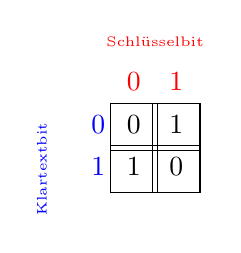
\begin{tikzpicture}[scale=0.9]
			\foreach \i in {0,...,1} {
				\node at (-0.5,-\i*0.6) {\textcolor{Blue}{\strut \i}};
				\node at (\i*0.6,0.6) {\textcolor{Red}{\strut \i}};
				\foreach \j in {0,...,1} {
					\edef\k{\ifnum\numexpr\i+\j\relax>1
							\the\numexpr\i+\j-2\relax
						\else
							\the\numexpr\i+\j\relax
						\fi}
					\node[draw,minimum size=0.6cm,inner sep=0pt]
					at (\i*0.6,-\j*0.6) {\strut\k};
				}
			}
			\node at (0.3,1.2) {\tiny{\textcolor{Red}{Schlüsselbit}}};
			\node[rotate = 90] at (-1.3,-0.6) {\tiny{\textcolor{Blue}{Klartextbit}}};
		\end{tikzpicture}
		\caption{Binäre Vigenère-Tabelle ($\oplus$ / XOR-Operation)}
	\end{figure}
\end{frame}

\begin{frame}{Verschlüsselung mit der $\oplus$-Operation (XOR)}
	Die Verschlüsselung erfolgt Bit für Bit mittels der Operation $\oplus$ (auch \emph{XOR} oder exklusives ODER genannt):
	\begin{align*}
		0 \oplus 0 = 0 \qquad\text{und}\qquad 0 \oplus 1 = 1 \\
		1 \oplus 0 = 1 \qquad\text{und}\qquad 1 \oplus 1 = 0
	\end{align*}\pause
	
	\begin{myexample}[Verschlüsselungsbeispiel]
		Klartext $\textcolor{Blue}{101}$, Schlüssel $\textcolor{ForestGreen}{111}$:
		\begin{center}
			\begin{tabular}{cccc}
				       & \textcolor{Blue}{1}        & \textcolor{Blue}{0}        & \textcolor{Blue}{1}        \\
				\oplus & \textcolor{ForestGreen}{1} & \textcolor{ForestGreen}{1} & \textcolor{ForestGreen}{1} \\
				\hline
				       & \textcolor{Red}{0}         & \textcolor{Red}{1}         & \textcolor{Red}{0}
			\end{tabular}
		\end{center}
		Somit ist der Kryptotext $\textcolor{Red}{010}$.
	\end{myexample}
\end{frame}

\begin{frame}{Mathematische Eigenschaften der $\oplus$-Operation}
	Für beliebige binäre Folgen $a, b, c$ gleicher Länge gelten folgende Gesetze:
	
	\begin{itemize}[<+->]
		\item \textbf{Kommutativität}: 
		      \[ a \oplus b = b \oplus a \]
		\item \textbf{Selbstinversität} (Verschlüsselung mit sich selbst ergibt $0$): 
		      \[ a \oplus a = 0 \]
		\item \textbf{Neutrales Element} (Verschlüsselung mit Nullen verändert nichts): 
		      \[ a \oplus 0 = a \]
		\item \textbf{Assoziativität}: 
		      \[ (a \oplus b) \oplus c = a \oplus (b \oplus c) \]
	\end{itemize}
\end{frame}

\begin{frame}{Warum funktioniert die Entschlüsselung?}
	Sei $t$ der Klartext und $s$ ein zufälliger geheimer Schlüssel.
	
	\begin{itemize}[<+->]
		\item \textbf{Verschlüsselung}: $c = t \oplus s$
		\item \textbf{Entschlüsselung} (erneute Anwendung desselben Schlüssels $s$):
		      \begin{align*}
			      c \oplus s & = (t \oplus s) \oplus s \\
			                 & = t \oplus (s \oplus s) \quad \text{(Assoziativität)} \\
			                 & = t \oplus 0 \qquad\quad \text{(Selbstinversität: } s \oplus s = 0\text{)} \\
			                 & = t \qquad\qquad\quad \text{(Neutrales Element: } t \oplus 0 = t\text{)}
		      \end{align*}
	\end{itemize}
	\pause
	Die erneute Anwendung des Schlüssels hebt die Verschlüsselung vollständig auf!
\end{frame}

\begin{frame}{Auftrag: Bin-OTP}
	\begin{itemize}
		\item \aufgabebox{Aufgaben 2.18-2.21}
		\item Zeit: 15 Minuten
		\item Danach: Gemeinsame Besprechung der Lösungen
	\end{itemize}
\end{frame}

% \begin{frame}{Problem: Schlüsselaustausch über unsichere Kanäle}
	\begin{myidea}[Schlüsseltausch ohne gemeinsamen Geheimschlüssel]
		Wie können Alice und Bob vertraulich kommunizieren, wenn sie vorab keinen gemeinsamen geheimen Schlüssel vereinbart haben?
	\end{myidea}
	
	\pause
	\vspace{0.2cm}
	\begin{block}{Die Kisten-Analogie (Truhe mit zwei Schlössern)}
		{\small
		\begin{enumerate}[<+->]
			\item Alice legt Klartext in eine Truhe, verschliesst sie mit Schloss $A$ und schickt sie an Bob.
			\item Bob schliesst zusätzlich sein eigenes Schloss $B$ an und schickt die Truhe zurück.
			\item Alice entfernt ihr Schloss $A$ und schickt die Truhe erneut an Bob.
			\item Bob entfernt sein Schloss $B$ und öffnet die Truhe.
		\end{enumerate}
		}
	\end{block}
\end{frame}

\begin{frame}
	\begin{myprocedure}[Three-Pass Protocol mit Bin-OTP]
		{\small
		Alice hat Schlüssel $s_A$, Bob Schlüssel $s_B$. Alice will Klartext \textcolor{Blue}{$t$} senden.
		
		\begin{enumerate}[<+->]
			\item \textbf{Schritt 1}: Alice verschlüsselt \textcolor{Blue}{$t$} mit $s_A$ ($k_A \rightarrow$ Bob):
			      \[ k_A = \textcolor{Blue}{t} \oplus \textcolor{Red}{s_A} \]
			\item \textbf{Schritt 2}: Bob verschlüsselt $k_A$ mit $s_B$ ($k_{AB} \rightarrow$ Alice):
			      \[ k_{AB} = k_A \oplus \textcolor{ForestGreen}{s_B} = \textcolor{Blue}{t} \oplus \textcolor{Red}{s_A} \oplus \textcolor{ForestGreen}{s_B} \]
			\item \textbf{Schritt 3}: Alice entfernt $s_A$ ($k_B \rightarrow$ Bob):
			      \[ k_B = k_{AB} \oplus \textcolor{Red}{s_A} = \textcolor{Blue}{t} \oplus \textcolor{ForestGreen}{s_B} \]
			\item \textbf{Schritt 4}: Bob entfernt $s_B$ und erhält den Klartext:
			      \[ \textcolor{Blue}{t} = k_B \oplus \textcolor{ForestGreen}{s_B} \]
		\end{enumerate}
		}
	\end{myprocedure}
\end{frame}

\begin{frame}{Beispiel: Drei-Wege-Schlüsseltausch}
	\begin{exampleblock}{Rechenbeispiel}
		Klartext $\textcolor{Blue}{t = 1100}$, Schlüssel Alice $\textcolor{Red}{s_A = 1011}$, Schlüssel Bob $\textcolor{ForestGreen}{s_B = 0110}$.
		\begin{center}
			\small
			\begin{tabular}{c|l|c}
				Schritt & Berechnung & Ergebnis \\ \hline
				1 (Alice $\rightarrow$ Bob) & $k_A = \textcolor{Blue}{1100} \oplus \textcolor{Red}{1011}$ & $0111$ \\
				2 (Bob $\rightarrow$ Alice) & $k_{AB} = 0111 \oplus \textcolor{ForestGreen}{0110}$ & $0001$ \\
				3 (Alice $\rightarrow$ Bob) & $k_B = 0001 \oplus \textcolor{Red}{1011}$ & $1010$ \\
				4 (Bob liest Klartext) & $t = 1010 \oplus \textcolor{ForestGreen}{0110}$ & $\textcolor{Blue}{1100}$
			\end{tabular}
		\end{center}
	\end{exampleblock}
\end{frame}

\begin{frame}{Sicherheit des Drei-Wege-Schlüsseltauschs}
	Ist das Drei-Wege-Protokoll mit XOR wirklich sicher?
	
	\pause
	\begin{alertblock}{Angriff durch Eve (Passives Abhören)}
		{\small
		Fängt Eve alle 3 Nachrichten ($k_A, k_{AB}, k_B$) ab, berechnet sie den Klartext $\textcolor{Blue}{t}$:
		\begin{align*}
			k_A \oplus k_{AB} \oplus k_B & = (\textcolor{Blue}{t} \oplus \textcolor{Red}{s_A}) \oplus (\textcolor{Blue}{t} \oplus \textcolor{Red}{s_A} \oplus \textcolor{ForestGreen}{s_B}) \oplus (\textcolor{Blue}{t} \oplus \textcolor{ForestGreen}{s_B}) \\
			                             & = \textcolor{Blue}{t} \oplus (\textcolor{Red}{s_A} \oplus \textcolor{Red}{s_A}) \oplus (\textcolor{ForestGreen}{s_B} \oplus \textcolor{ForestGreen}{s_B}) = \textcolor{Blue}{t}
		\end{align*}
		}
	\end{alertblock}
	
	\pause
	\textbf{Fazit}: Das XOR-basierte Protokoll schützt nicht vor einem Abhörer!
\end{frame}

\begin{frame}{Auftrag: Drei-Wege-Schlüsseltausch}
	\begin{itemize}
		\item \aufgabebox{Lösen Sie Aufgabe 3.1 im Skript zu zweit.}
		\item Zeit: 10 Minuten
	\end{itemize}
\end{frame}

% \begin{frame}{Diffie-Hellman-Merkle-Schlüsseltausch (DHM)}
	1976 erfanden Whitfield Diffie, Martin Hellman und Ralph Merkle das erste Verfahren für einen sicheren Schlüsselaustausch über unsichere Kanäle.
	
	\begin{myidea}[Diskretes Logarithmusproblem]
		Das Verfahren basiert auf einer mathematischen \textbf{Einwegfunktion} modulo einer Primzahl $p$:
		\begin{itemize}[<+->]
			\item \textbf{Einfach}: $x = g^a \bmod p$ berechnen.
			\item \textbf{Sehr schwer}: Aus $x, g, p$ den geheimen Exponenten $a$ zurückrechnen (\emph{Diskreter Logarithmus}).
		\end{itemize}
	\end{myidea}
\end{frame}

\begin{frame}{Ablauf des DHM-Protokolls}
	\begin{myprocedure}[Protokoll \acrshort{DHM}]
		{\small
		Öffentlich vereinbarte Werte: Primzahl $p$ und Basis $g < p$.
		
		\begin{enumerate}[<+->]
			\item \textbf{Alice}: Wählt geheime Zahl $a < p$. Berechnet $x := g^a \bmod p$ und sendet $x$ an Bob.
			\item \textbf{Bob}: Wählt geheime Zahl $b < p$. Berechnet $y := g^b \bmod p$ und sendet $y$ an Alice.
			\item \textbf{Alice} berechnet gemeinsamen Schlüssel:
			      $s_{AB} := y^a \bmod p$.
			\item \textbf{Bob} berechnet gemeinsamen Schlüssel:
			      $s_{AB} := x^b \bmod p$.
		\end{enumerate}
		}
	\end{myprocedure}
\end{frame}

\begin{frame}{Warum erhalten beide denselben Schlüssel?}
	Aus den Potenzgesetzen folgt:
	\[ (g^b)^a \bmod p = g^{b \cdot a} \bmod p = g^{a \cdot b} \bmod p = (g^a)^b \bmod p \]
	
	\pause
	\begin{align*}
		\text{Alice berechnet: } & y^a \bmod p = (g^b)^a \bmod p = \mathbf{g^{ab} \bmod p} \\
		\text{Bob berechnet: }   & x^b \bmod p = (g^a)^b \bmod p = \mathbf{g^{ab} \bmod p}
	\end{align*}
	
	\pause
	\begin{alertblock}{Was sieht der Abhörer Eve?}
		Eve sieht nur $p, g, x, y$. Ohne $a$ oder $b$ kann Eve $g^{ab} \bmod p$ nicht berechnen!
	\end{alertblock}
\end{frame}

\begin{frame}{Rechenbeispiel: DHM-Schlüsseltausch}
	\begin{exampleblock}{Beispiel mit kleinen Zahlen}
		Öffentliche Parameter: $p = 13$, $g = 2$.
		
		\begin{enumerate}[<+->]
			\item \textbf{Alice} ($a = 5$):
			      $x = 2^5 \bmod 13 = 32 \bmod 13 = 6$
			\item \textbf{Bob} ($b = 4$):
			      $y = 2^4 \bmod 13 = 16 \bmod 13 = 3$
			\item \textbf{Alice}:
			      $s_{AB} = y^a \bmod p = 3^5 \bmod 13 = 243 \bmod 13 = \mathbf{9}$
			\item \textbf{Bob}:
			      $s_{AB} = x^b \bmod p = 6^4 \bmod 13 = 1296 \bmod 13 = \mathbf{9}$
		\end{enumerate}
	\end{exampleblock}
\end{frame}

\begin{frame}{Auftrag: Diffie-Hellman-Merkle}
	\begin{itemize}
		\item \aufgabebox{Lösen Sie die Aufgaben 3.2, 3.3 und 3.4 im Skript}
		\item Zeit: 15 Minuten
	\end{itemize}
\end{frame}

